\documentclass[aspectratio=169,11pt]{beamer}
\usepackage[utf8]{inputenc}
\usepackage[T1]{fontenc}
\usepackage[french]{babel}
\usepackage{amsmath,amssymb}
\usepackage{booktabs}
\usepackage{graphicx}
\usepackage{array}

\usetheme{Madrid}
\usecolortheme{default}
\setbeamertemplate{navigation symbols}{}
\setbeamertemplate{caption}[numbered]

\definecolor{mainblue}{RGB}{24,64,122}
\definecolor{accent}{RGB}{190,70,50}
\setbeamercolor{structure}{fg=mainblue}
\setbeamercolor{frametitle}{bg=mainblue,fg=white}
\setbeamercolor{title}{fg=mainblue}

\title[ICA stochastique]{Implementation et evaluation de methodes ICA classiques et stochastiques}
\author{Abdoulaye Diallo}
\date{4 avril 2026}

\begin{document}

\begin{frame}
  \titlepage
\end{frame}

\begin{frame}{Message principal}
  \begin{itemize}
    \item Objectif: comparer FastICA, SGD-ICA et Adam-ICA sur des donnees ICA synthetiques.
    \item Trois axes: scalabilite, convergence, robustesse au bruit.
    \item Contribution complementaire: effet de la non-gaussianite des sources.
  \end{itemize}

  \vspace{0.5em}
  \begin{block}{Conclusion executive}
    FastICA reste la reference la plus fiable en precision sur les tests realises; les variantes stochastiques sont surtout interessantes pour l'analyse de convergence et certains compromis temps/qualite.
  \end{block}
\end{frame}

\begin{frame}{Protocole experimental}
  \begin{columns}[T,onlytextwidth]
    \column{0.52\textwidth}
    \begin{block}{Modele}
      \[
      x = As, \qquad y = Vx
      \]
      \begin{itemize}
        \item Sources synthetiques independantes.
        \item Pretraitement: centrage + whitening.
        \item Evaluation: indice d'Amari.
      \end{itemize}
    \end{block}

    \column{0.48\textwidth}
    \begin{block}{Algorithmes}
      \begin{itemize}
        \item FastICA: reference sklearn.
        \item SGD-ICA: Infomax mini-batch.
        \item Adam-ICA: Infomax avec moments adaptatifs.
      \end{itemize}
      \vspace{0.3em}
      \small
      Plus l'Amari est bas, meilleure est la separation.
    \end{block}
  \end{columns}
\end{frame}

\begin{frame}{Scalabilite}
  \small
  \begin{columns}[T,onlytextwidth]
    \column{0.5\textwidth}
    \textbf{Variation en dimension} (N = 5000, moyenne sur 3 seeds)
    \vspace{0.4em}

    \resizebox{\linewidth}{!}{%
    \begin{tabular}{lcc}
      \toprule
      Algo & Amari $D=3\rightarrow40$ & Temps $D=3\rightarrow40$ \\
      \midrule
      FastICA & 0.0124 $\rightarrow$ 0.0129 & 0.014s $\rightarrow$ 0.584s \\
      SGD-ICA & 0.1516 $\rightarrow$ 0.3044 & 0.521s $\rightarrow$ 14.315s \\
      Adam-ICA & 0.3073 $\rightarrow$ 0.3116 & 0.488s $\rightarrow$ 12.151s \\
      \bottomrule
    \end{tabular}%
    }

    \vspace{0.8em}
    \textbf{Variation en N} (D = 20, epochs fixes)
    \vspace{0.4em}

    \resizebox{\linewidth}{!}{%
    \begin{tabular}{lcc}
      \toprule
      Algo & Amari $N=1000\rightarrow10000$ & Temps $N=1000\rightarrow10000$ \\
      \midrule
      FastICA & 0.0289 $\rightarrow$ 0.0089 & 0.067s $\rightarrow$ 0.470s \\
      SGD-ICA & 0.3451 $\rightarrow$ 0.3206 & 0.085s $\rightarrow$ 9.542s \\
      Adam-ICA & 0.3474 $\rightarrow$ 0.3294 & 0.067s $\rightarrow$ 8.646s \\
      \bottomrule
    \end{tabular}%
    }

    \column{0.46\textwidth}
    \begin{block}{Lecture rapide}
      \begin{itemize}
        \item FastICA garde une excellente precision sur toute la plage testee.
        \item Les methodes stochastiques restent plus sensibles aux hyperparametres.
        \item Le cout calcul augmente plus vite pour SGD/Adam sur ces reglages.
      \end{itemize}
    \end{block}
  \end{columns}
\end{frame}

\begin{frame}{Convergence}
  \begin{columns}[T,onlytextwidth]
    \column{0.62\textwidth}
    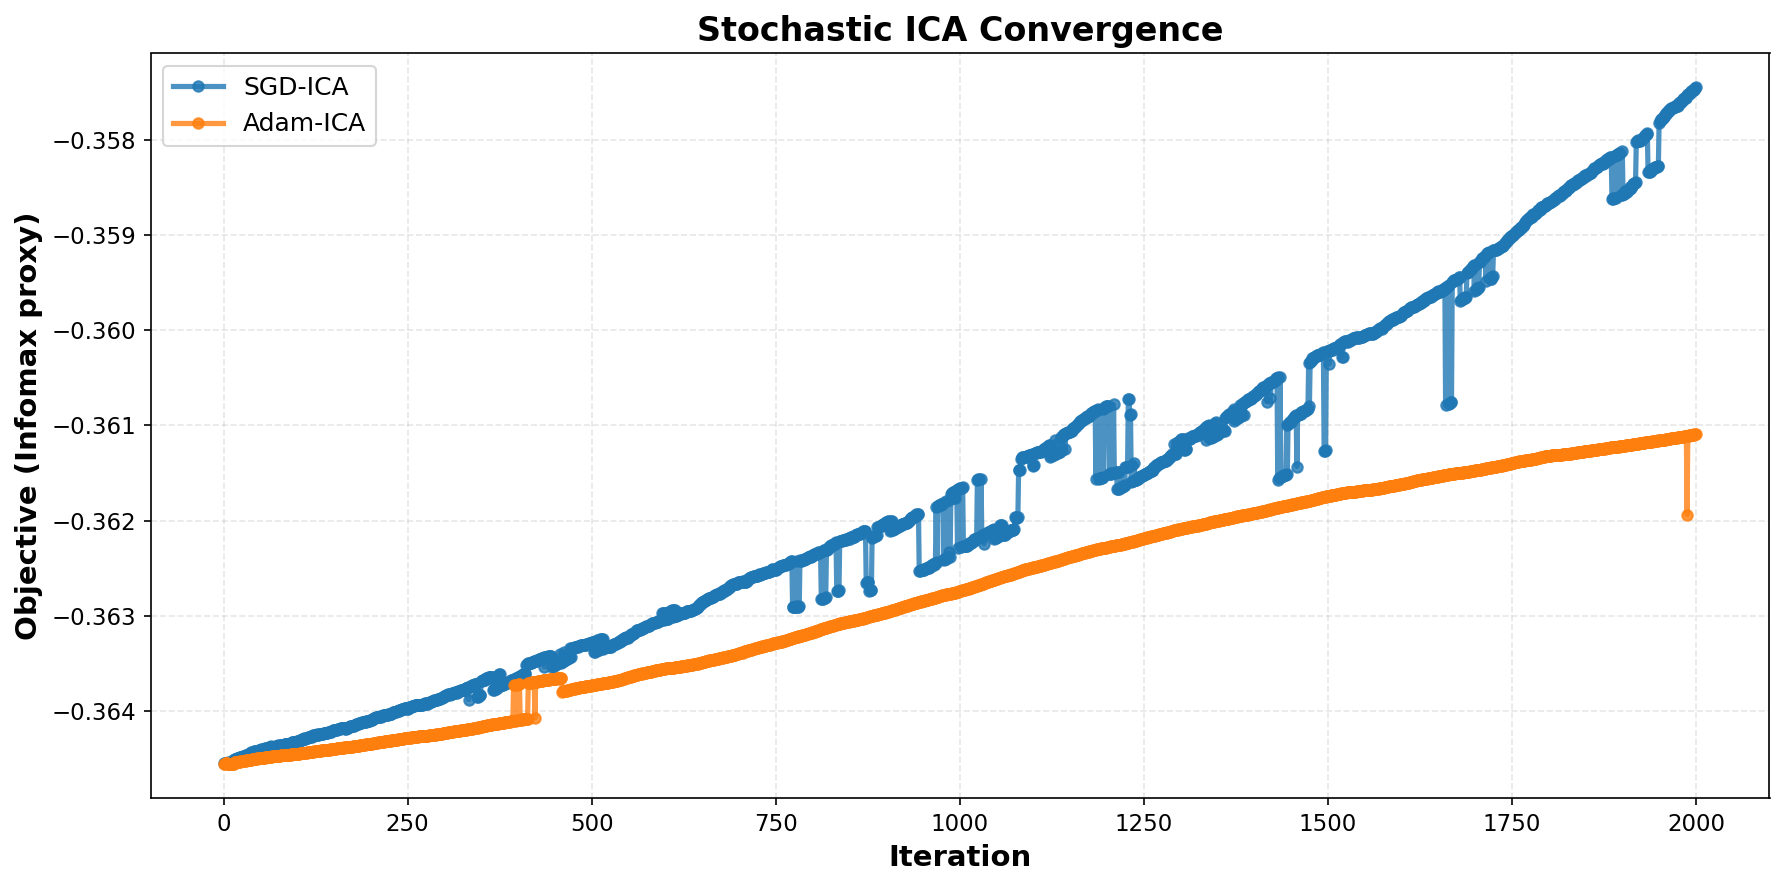
\includegraphics[width=\textwidth]{../results/convergence_plot.png}

    \column{0.38\textwidth}
    \begin{block}{Points cles}
      \begin{itemize}
        \item SGD-ICA progresse plus nettement sur l'objectif Infomax.
        \item Adam-ICA evolue plus lentement avec le reglage retenu.
        \item La dynamique d'optimisation depend fortement du pas et du mini-batch.
      \end{itemize}
    \end{block}
  \end{columns}
\end{frame}

\begin{frame}{Robustesse au bruit}
  \begin{columns}[T,onlytextwidth]
    \column{0.62\textwidth}
    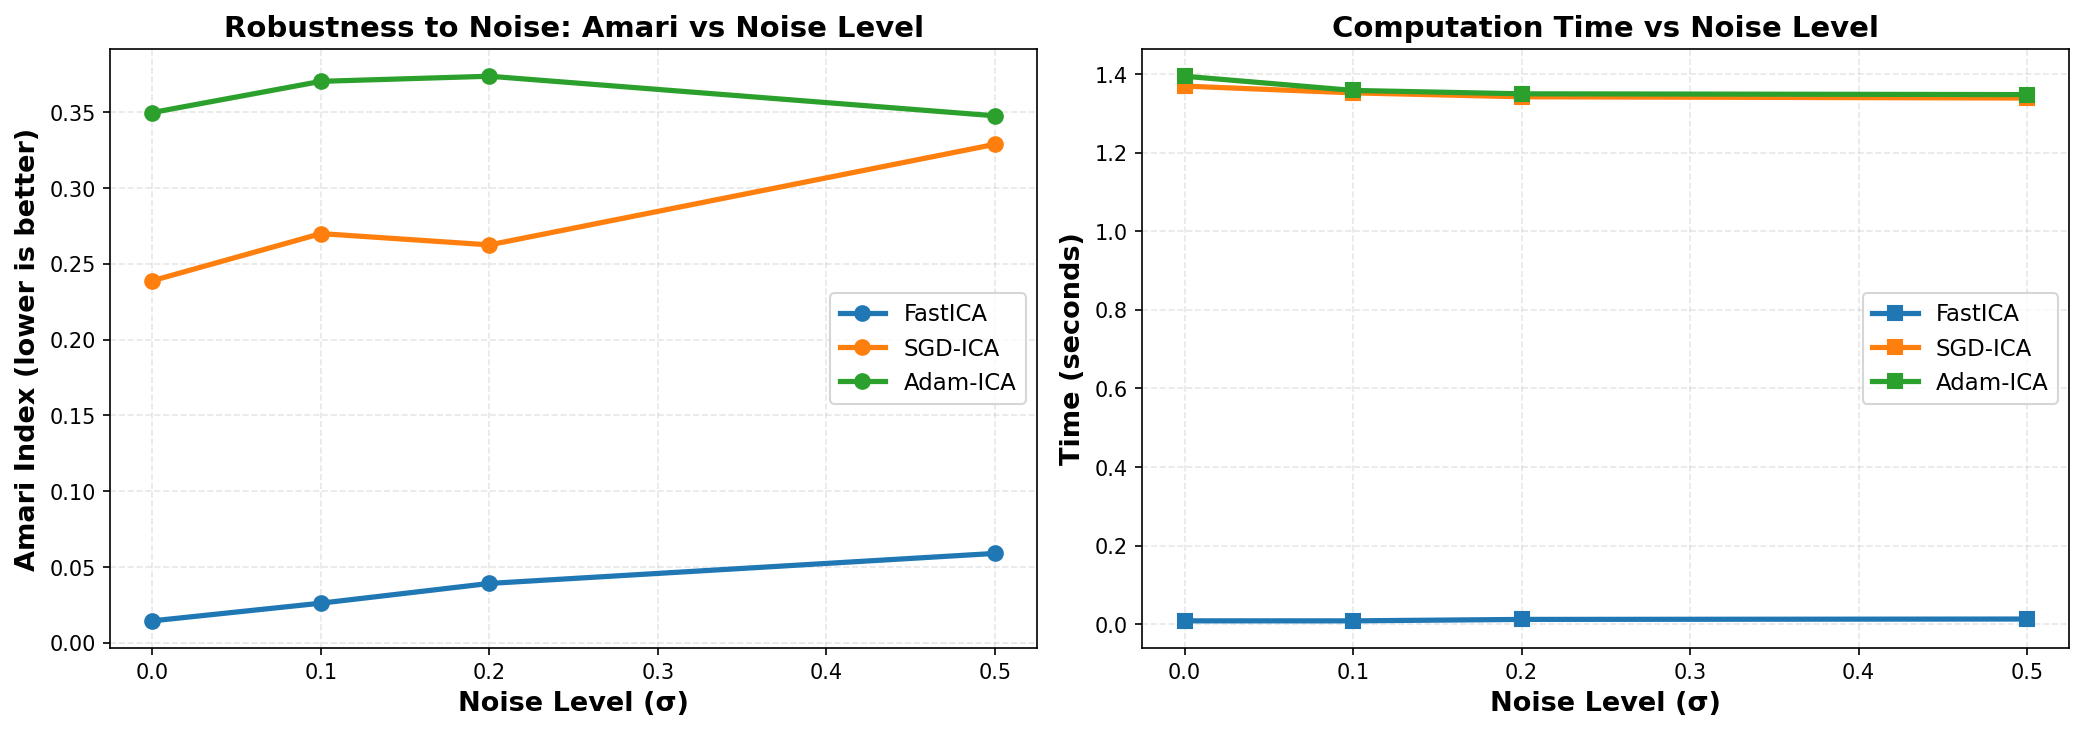
\includegraphics[width=\textwidth]{../results/noise_robustness_plot.png}

    \column{0.38\textwidth}
    \begin{block}{Lecture rapide}
      \begin{itemize}
        \item FastICA reste la methode la plus precise quand le bruit augmente.
        \item Les methodes stochastiques se degradent plus vite.
        \item SGD-ICA garde un leger avantage sur Adam-ICA dans certains regimes bruyants.
      \end{itemize}
    \end{block}
  \end{columns}
\end{frame}

\begin{frame}{Contribution creative: gaussianite des sources}
  \begin{itemize}
    \item Le notebook \texttt{gaussian\_problem.ipynb} explore l'impact du parametre de forme $\alpha$ d'une gaussienne generalisee.
    \item Message observe: la zone la plus sensible est le voisinage de $\alpha=2$.
    \item L'indice d'Amari se degrade nettement quand les sources deviennent proches du cas gaussien.
    \item La conclusion reste stable: la non-gaussianite n'est pas un detail, c'est une condition structurante de l'ICA.
  \end{itemize}

  \begin{block}{Interpretation}
    Cette partie donne une lecture plus mecaniste des performances: le comportement algorithmique depend autant du contraste choisi que de la statistique des sources.
  \end{block}
\end{frame}

\begin{frame}{Kurtosis et gaussianite}
  \begin{columns}[T,onlytextwidth]
    \column{0.57\textwidth}
    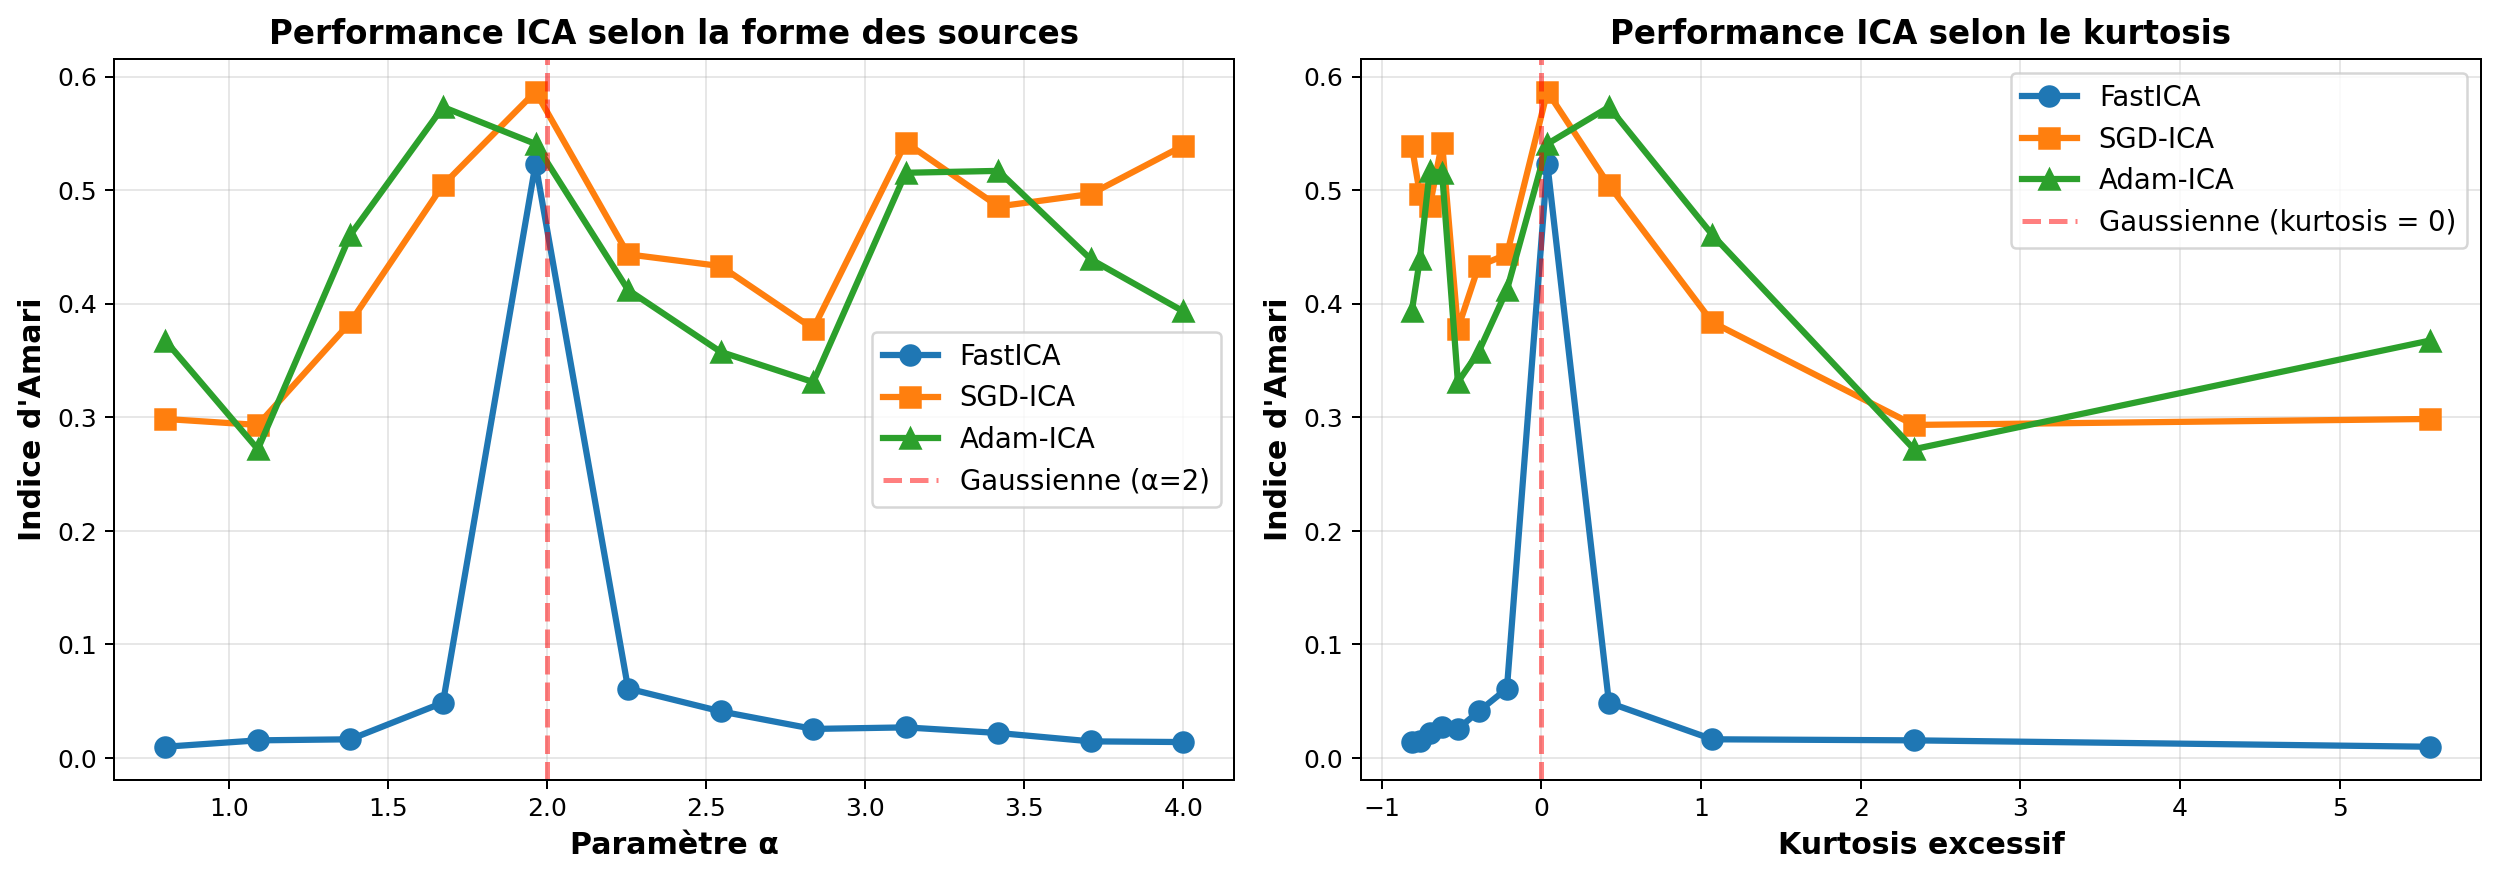
\includegraphics[width=\textwidth]{../results/kurtosis_impact.png}

    \column{0.43\textwidth}
    \begin{block}{Lecture}
      \begin{itemize}
        \item Le pire regime reste proche de $\alpha=2$ et du kurtosis nul.
        \item Les trois algorithmes suivent la meme structure globale.
        \item Les ecarts restants sont surtout algorithmiques, pas conceptuels.
      \end{itemize}
    \end{block}
  \end{columns}
\end{frame}

\begin{frame}{Formes de sources}
  \begin{columns}[T,onlytextwidth]
    \column{0.72\textwidth}
    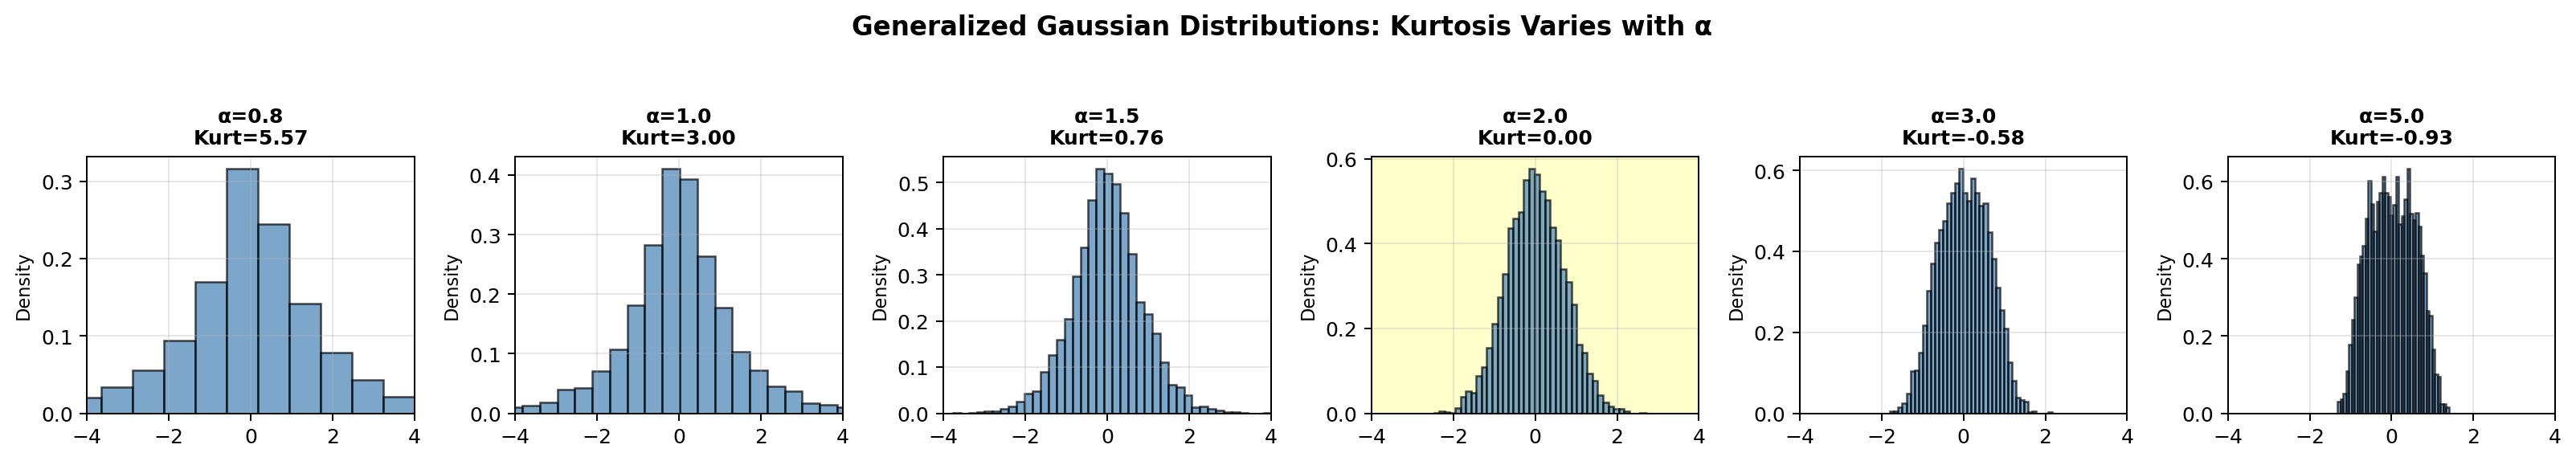
\includegraphics[width=\textwidth]{../results/gg_distributions.png}

    \column{0.28\textwidth}
    \begin{block}{Repere}
      \small
      \begin{itemize}
        \item $\alpha<2$ : queues lourdes.
        \item $\alpha=2$ : cas gaussien.
        \item $\alpha>2$ : distribution plus aplatie.
      \end{itemize}
    \end{block}
  \end{columns}
\end{frame}

\begin{frame}{Conclusion}
  \begin{itemize}
    \item FastICA est la baseline la plus robuste en precision sur les cas testes.
    \item Les methodes stochastiques sont utiles pour l'analyse de convergence et certains compromis de temps.
    \item La gaussianite des sources module fortement la difficulte du probleme ICA.
    \item Le projet est coherent de bout en bout: implementation, evaluation empirique et interpretation theorique.
  \end{itemize}

  \vspace{0.5em}
  \centering
  \Large Merci
\end{frame}

\end{document}